% Schema del modello definito in 01_network.py, disegnato nello stesso stile dei
% diagrammi di 05_gpt/. Il flusso al centro e' la rete che il file costruisce
% davvero; le note a destra dicono cosa faceva il capitolo 1 di Nielsen nello
% stesso punto, e perche' qui si fa altro.
%
% Compilare con:
%     tectonic 01_out_architecture.tex
%     pdflatex 01_out_architecture.tex
%
% Per riusarlo dentro un altro documento: copiare le \definecolor, la lista di
% stili e il blocco tikzpicture, lasciando perdere il resto del preambolo.

\documentclass[tikz,border=8pt]{standalone}

\usepackage[T1]{fontenc}
\usepackage{lmodern}
\usetikzlibrary{positioning,fit,calc,arrows.meta,backgrounds}

% la stessa palette dei diagrammi di 05_gpt
\definecolor{cIn}{RGB}{248,214,216}
\definecolor{cAct}{RGB}{252,224,187}
\definecolor{cLin}{RGB}{216,214,238}
\definecolor{cLoss}{RGB}{205,235,205}
\definecolor{cBlk}{RGB}{240,240,240}

\begin{document}
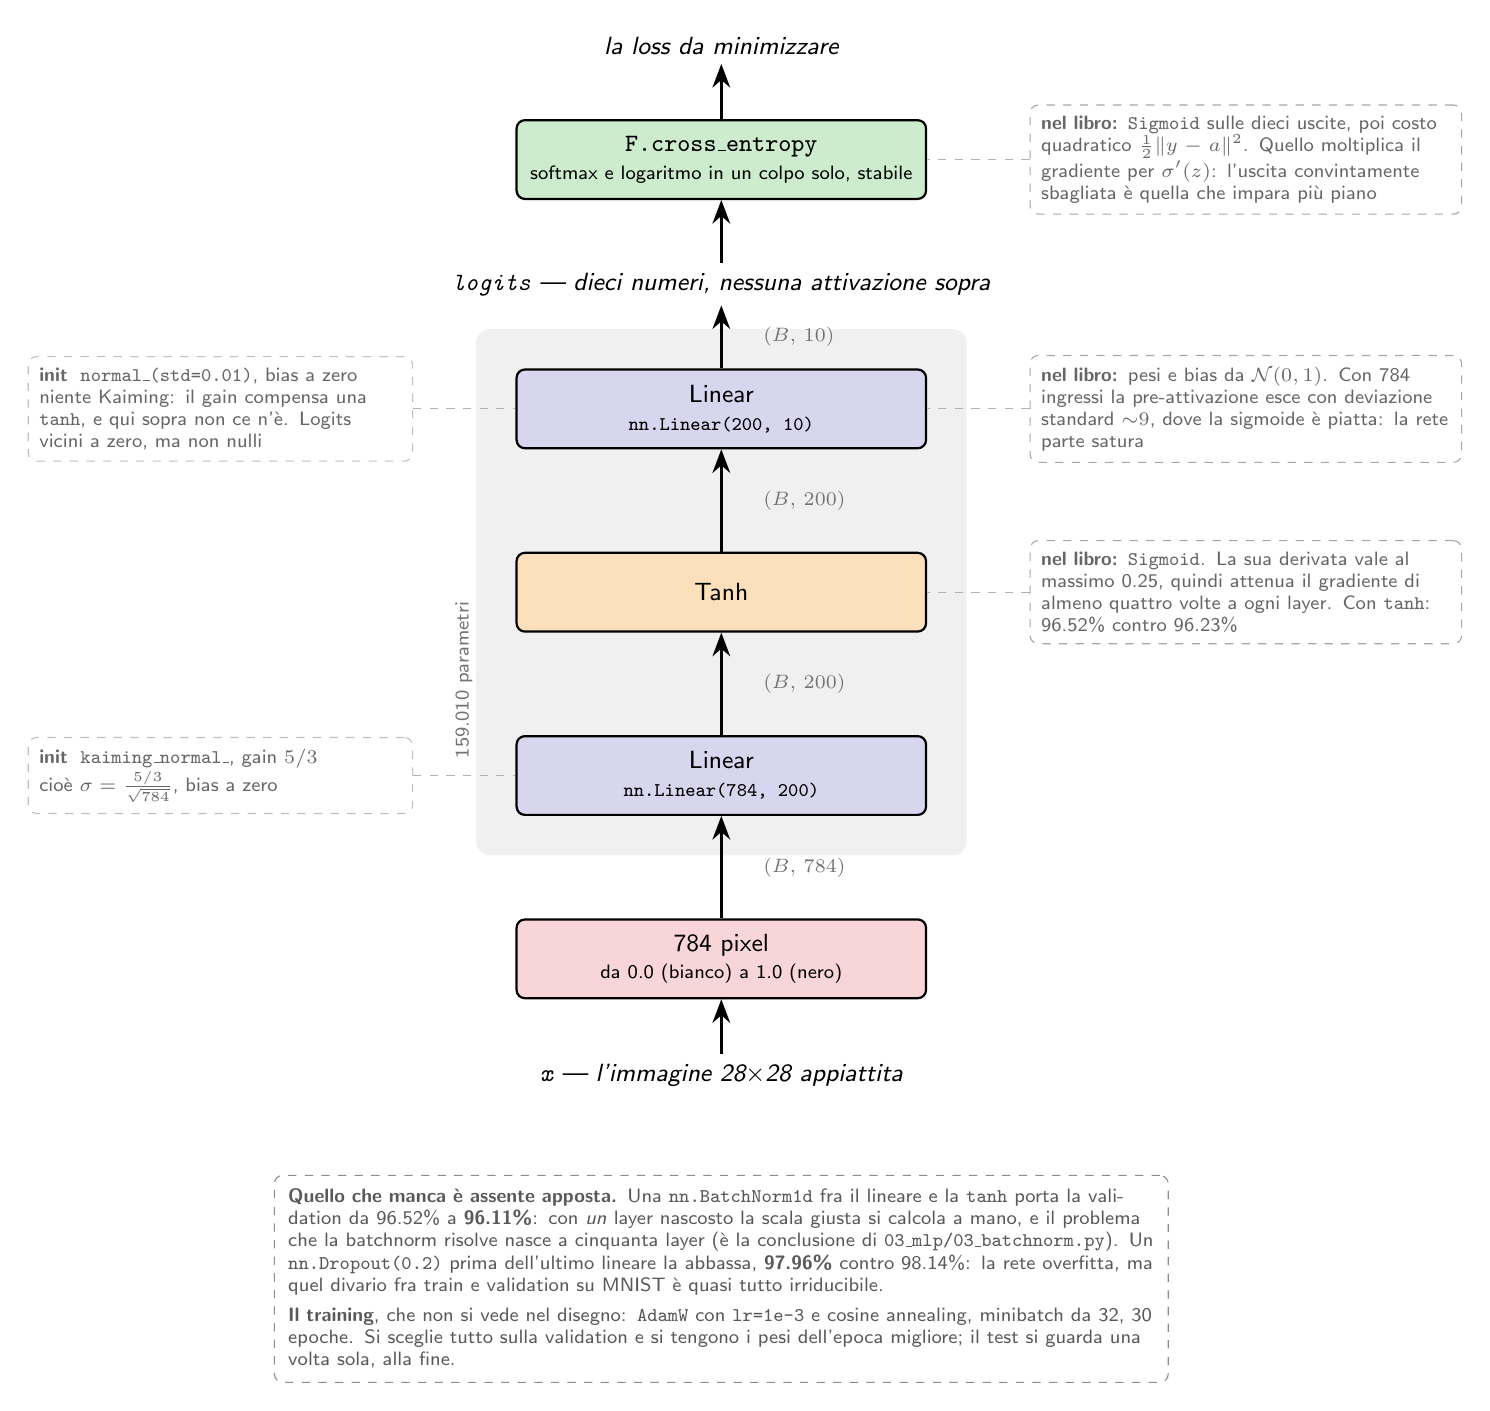
\begin{tikzpicture}[
  font=\sffamily\small,
  box/.style   = {draw, thick, rounded corners=3pt, align=center,
                  minimum width=52mm, minimum height=10mm, inner sep=3pt},
  io/.style    = {align=center, font=\sffamily\small\itshape},
  flow/.style  = {-{Stealth[length=3mm]}, line width=0.9pt},
  shp/.style   = {font=\sffamily\scriptsize, text=black!55,
                  anchor=west, xshift=4mm},
  book/.style  = {draw=black!35, dashed, rounded corners=3pt, align=left,
                  font=\sffamily\scriptsize, text=black!60, inner sep=4pt,
                  text width=52mm},
  note/.style  = {draw=black!45, dashed, rounded corners=3pt, align=left,
                  font=\sffamily\scriptsize, text=black!65, inner sep=5pt}
]

% ---------------------------------------------------------------- il flusso --
\node[io]                                    (inp)  {\texttt{x} \textemdash{} l'immagine 28$\times$28 appiattita};
\node[box, fill=cIn, above=7mm of inp]       (pix)  {784 pixel\\[-1pt]{\scriptsize da 0.0 (bianco) a 1.0 (nero)}};
\node[box, fill=cLin, above=13mm of pix]     (l1)   {Linear\\[-1pt]{\scriptsize\texttt{nn.Linear(784, 200)}}};
\node[box, fill=cAct, above=13mm of l1]      (act)  {Tanh};
\node[box, fill=cLin, above=13mm of act]     (l2)   {Linear\\[-1pt]{\scriptsize\texttt{nn.Linear(200, 10)}}};
\node[io, above=8mm of l2]                   (log)  {\texttt{logits} \textemdash{} dieci numeri, nessuna attivazione sopra};
\node[box, fill=cLoss, above=8mm of log]     (loss) {\texttt{F.cross\_entropy}\\[-1pt]{\scriptsize softmax e logaritmo in un colpo solo, stabile}};
\node[io, above=7mm of loss]                 (outp) {la loss da minimizzare};

% ------------------------------------------------------------------- archi --
\draw[flow] (inp)  -- (pix);
\draw[flow] (pix)  -- (l1)   node[shp, midway] {$(B,\,784)$};
\draw[flow] (l1)   -- (act)  node[shp, midway] {$(B,\,200)$};
\draw[flow] (act)  -- (l2)   node[shp, midway] {$(B,\,200)$};
\draw[flow] (l2)   -- (log)  node[shp, midway] {$(B,\,10)$};
\draw[flow] (log)  -- (loss);
\draw[flow] (loss) -- (outp);

% ----------------------------------------------- come parte ogni layer, a sx --
\node[book, left=13mm of l1, text width=46mm, draw=black!25] (i1) {%
  \textbf{init}\; \texttt{kaiming\_normal\_}, gain $5/3$\\
  cio\`e $\sigma = \frac{5/3}{\sqrt{784}}$, bias a zero};
\node[book, left=13mm of l2, text width=46mm, draw=black!25] (i2) {%
  \textbf{init}\; \texttt{normal\_(std=0.01)}, bias a zero\\
  niente Kaiming: il gain compensa una \texttt{tanh}, e qui sopra non ce n'\`e.
  Logits vicini a zero, ma non nulli};
\draw[dashed, black!30] (i1) -- (l1);
\draw[dashed, black!30] (i2) -- (l2);

% ------------------------------------------------- cosa faceva il libro, a dx --
\node[book, right=13mm of act] (b1) {%
  \textbf{nel libro:} \texttt{Sigmoid}. La sua derivata vale al massimo 0.25,
  quindi attenua il gradiente di almeno quattro volte a ogni layer.
  Con \texttt{tanh}: 96.52\% contro 96.23\%};
\node[book, right=13mm of l2] (b2) {%
  \textbf{nel libro:} pesi e bias da $\mathcal{N}(0,1)$. Con 784 ingressi la
  pre-attivazione esce con deviazione standard ${\sim}9$, dove la sigmoide
  \`e piatta: la rete parte satura};
\node[book, right=13mm of loss] (b3) {%
  \textbf{nel libro:} \texttt{Sigmoid} sulle dieci uscite, poi costo
  quadratico $\frac{1}{2}\|y-a\|^2$. Quello moltiplica il gradiente
  per $\sigma'(z)$: l'uscita convintamente sbagliata \`e quella che impara
  pi\`u piano};
\draw[dashed, black!30] (b1) -- (act);
\draw[dashed, black!30] (b2) -- (l2);
\draw[dashed, black!30] (b3) -- (loss);

% ------------------------------------------- il pezzo che il training aggiunge --
\begin{scope}[on background layer]
  \node[fill=cBlk, rounded corners=5pt, fit=(l1)(act)(l2), inner sep=5mm] (net) {};
\end{scope}
\node[font=\sffamily\scriptsize, text=black!55, rotate=90, left=1.5mm of net]
  {159.010 parametri};

% -------------------------------------------------------- cosa non c'e', e perche' --
\node[note, below=10mm of inp, text width=110mm] (nota) {%
  \textbf{Quello che manca \`e assente apposta.} Una \texttt{nn.BatchNorm1d} fra
  il lineare e la \texttt{tanh} porta la validation da 96.52\% a \textbf{96.11\%}:
  con \emph{un} layer nascosto la scala giusta si calcola a mano, e il problema
  che la batchnorm risolve nasce a cinquanta layer
  (\`e la conclusione di \texttt{03\_mlp/03\_batchnorm.py}). Un
  \texttt{nn.Dropout(0.2)} prima dell'ultimo lineare la abbassa,
  \textbf{97.96\%} contro 98.14\%: la rete overfitta, ma quel divario fra train e
  validation su MNIST \`e quasi tutto irriducibile.\\[3pt]
  \textbf{Il training}, che non si vede nel disegno: \texttt{AdamW} con
  \texttt{lr=1e-3} e cosine annealing, minibatch da 32, 30 epoche. Si sceglie
  tutto sulla validation e si tengono i pesi dell'epoca migliore;
  il test si guarda una volta sola, alla fine.};

\end{tikzpicture}
\end{document}
